\documentclass[letterpaper]{article}
\usepackage{aaai}
\usepackage{times,helvet,courier}
\usepackage{color}
\usepackage{tikz}
\usepackage{graphicx}

\frenchspacing

\setlength{\pdfpagewidth}{8.5in}
\setlength{\pdfpageheight}{11in}
\setcounter{secnumdepth}{0}  

\pdfinfo{
/Title (Information Shaping for Robot Planning)
/Author (Michael Cashmore, Sarah Keren)}


%= TIKZ =%
\tikzstyle myBG=[line width=3pt,opacity=1]
\newcommand{\drawLinewithBG}[2]
{
  \draw[white,myBG]  (#1) -- (#2);
  \draw[black,very thick] (#1) -- (#2);
}
\newcommand{\drawPolarLinewithBG}[2]
{
  \draw[white,myBG]  (#1) -- (#2);
  \draw[black,very thick] (#1) -- (#2);
}

\begin{document}

\title{Information Shaping for Robot Planning}
\author{
Michael Cashmore$^{1}$ \and Sarah Keren$^{2}$\\
$^{1}$ University of Strathclyde, Glasgow, UK, \textit{michael.cashmore@strath.ac.uk}\\
$^{2}$ Harvard University, United States, \textit{skeren@seas.harvard.edu}
}

\maketitle

% \begin{abstract}
% \begin{quote}
% \end{quote}
% \end{abstract}

% Authors are required to submit two items:
% (1) a 2-page short paper describing their system, formatted in AAAI two-column style, and
% (2) a video (of duration up to 10 minutes) of the proposed demonstration.
% Slides are also permitted in lieu of video, but greater weight will be given to submissions accompanied by videos. The paper must present the technical details of the demonstration, discuss related work, and describe the significance of the demonstration. The paper must contain unpublished work. If accepted, authors will be required to transfer copyright of their paper to AAAI. For more information on the AAAI style, please download the AAAI Press author kit.

\section{Introduction}

%% MOTIVATION
We present a demonstration of using hidden costs for task planning and navigation.
%
A hidden cost is a cost that is not accounted for in the planner's model directly. In this demo we focus on hidden costs in navigation only. A hidden cost in this context could be an area of carpet upon which a low-profile robot is only able to move slowly, or is at risk of getting stuck. A cost could also be a user preference for the robot to avoid a certain area because it is a high-traffic area for humans. We combine navigation costs from multiple sources, including:
\begin{itemize}
    \item Areas in which navigation is particularly difficult.
    \item Costs that favour areas where the intention of the robot is easier to discern.
    \item Costs that favour areas of higher utility.
    \item Costs that are derived from social norms, such as avoiding areas that block human traffic.
\end{itemize}
%
Importantly a robot that enters the environment for the first time is not aware of these costs. The robot's model of the environment is in two parts: (a) the task planning model (consisting of a domain model and an initial configuration, including goal) and (b) data that can be sensed or requested by the robot but is not included in the planning model, such as the occupancy grid and the navigational cost map.

In order for the hidden costs to alter the behaviour of the robot, the costs must be embedded into the information already available. Our system does this in two ways:
\begin{enumerate}
    \item \textit{Cost-based Discretisation}, and
    \item \textit{Combined Costmaps for navigation}.
\end{enumerate}
Using a combination of these techniques the robot is able to generate more efficient solutions, solve more problems, and behave in a more preferable way with respect the hidden costs.

% screenshot of the stage demo
\begin{figure}[!th]
    \centering
    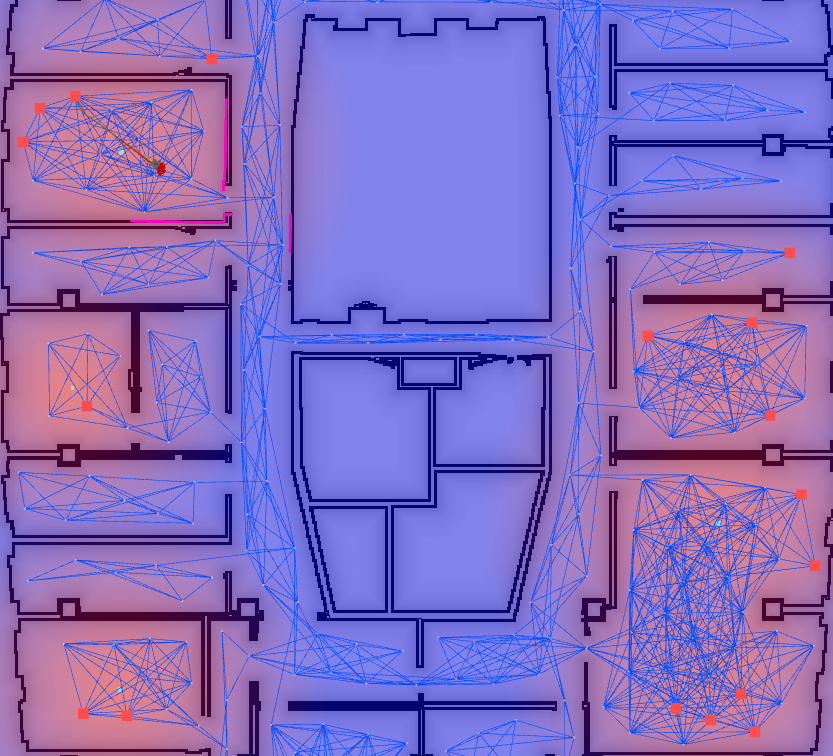
\includegraphics[width=0.4\textwidth]{screenshot_heatmap.png}
    \caption{Screenshot of the robot visualisation showing the static map (in black) the complete probabilistic roadmap (blue edges) the combined costmaps of the hidden cost (as a heatmap) and the sampled waypoints (red squares).}
    \label{fig:my_label}
\end{figure}
\section{Background}

The problem of selecting which information to reveal, which we call {\em information shaping}, is challenging because the space of information shaping options may be extremely large, and because more information need not make an agent's intention easier to recognize, or even help the robot achieve a better utility.
Our interest here is in modulating the behavior of the robot through information shaping. By changing the actor's knowledge, we can potentially change its behavior and the way by which it acquires the information needed to achieve it's goal.  We restrict the information shaping interventions to be truthful  so that they cannot convey false information.
In the context of contingent, partially-informed planning agents, this requirement is naturally implemented by requiring that we may only improve the actor's sensor model, i.e., improving its ability to  access the  value of some environment feature. 


\section{System Description}

\begin{figure*}[!th]
    \centering
    \usetikzlibrary[positioning,fit,shadings,shapes,backgrounds,arrows,calc]

\tikzstyle{node}=[rectangle,thick,draw=black!75,fill=white!20,minimum size=6mm]

\tikzset{*|/.style={to path={(perpendicular cs: horizontal line through={(\tikztostart)},vertical line through={(\tikztotarget)}) -- (\tikztotarget) \tikztonodes}}}

\begin{tikzpicture}[scale=0.85,every node/.style={scale=0.85}]

  \begin{scope}[local bounding box=orig](orig)
  
    \draw[black!25,very thick,dashed] (-1.5,-1) rectangle (1.5,-3);
    \draw[black!25,very thick,dashed] (2.5,1) rectangle (7.5,-3);
    
    \node at (-1.5,-2) (A) [text=black!40,anchor=south,rotate=90] {path planning};
    \node at (7.5,-1) (A) [text=black!40,anchor=north,rotate=90] {task planning};

    % nodes
    \node[node] at (0,0) (ms) {map server};
    \node[node] at (5,0) (rg) {ROSPlan PRM generation};
    \node[node] at (5,-2) (rp) {ROSPlan};
    \node[node] at (0,-2) (mb) {movebase};
    \node[node] at (0,-4) (bc) {base controller};

    \draw[->,*|] (ms.south) to node[pos=0.25,left]{\textit{/map}} (mb.north);
    \draw[->] (ms.east) to node[pos=0.25,below]{\textit{/map}} (rg.west);
    \draw[->,*|] (rg.south) to node[pos=0.25,right]{\textit{/waypoints}} (rp.north);
    \draw[->] (rp.west) to node[pos=0.5,below]{\textit{/action\_dispatch}} (mb.east);
    \draw[->,*|] (mb.south) to node[pos=0.75,left]{\textit{/cmd\_vel}} (bc.north);

  \end{scope}

  \begin{scope}[xshift=32em,scale=0.9,every node/.style={scale=0.9}](new)
  
    % \draw[black!25,very thick,dashed] (-1.5,-3) rectangle (1.5,-5);
    % \draw[black!25,very thick,dashed] (2.5,1) rectangle (7.5,-5);
    
    % \node at (-1.5,-4) (A) [text=black!40,anchor=south,rotate=90] {path planning};
    % \node at (7.5,-1) (A) [text=black!40,anchor=north,rotate=90] {task planning};

    % nodes
    \node[node] at (0,0) (ms) {map server};
    \node[node] at (5,0) (rg) {ROSPlan PRM generation};
    \node[node] at (5,-2) (ws) [draw=red,text=red] {WP-Sampler};
    \node[node] at (5,-4) (rp) {ROSPlan};
    \node[node] at (0,-2) (sm) [draw=red,text=red] {enhanced map server};
    \node[node] at (0,-4) (mb) {movebase};
    \node[node] at (0,-6) (bc) {base controller};

    \draw[->,*|] (ms.south) to node[pos=0.25,left]{\textit{/map}} (sm.north);
    \draw[->,*|,draw=red] (sm.south) to node[pos=0.25,left,text=red]{\textit{/map'}} (mb.north);
    \draw[->] (ms.east) to node[pos=0.5,below]{\textit{/map}} (rg.west);
    \draw[->,*|] (rg.south) to node[pos=0.25,right]{\textit{/waypoints}} (ws.north);
    \draw[->,draw=red] (sm.east) to node[pos=0.5,below,text=red]{\textit{/map'}} (ws.west);
    \draw[->,*|,draw=red] (ws.south) to node[pos=0.25,right,text=red]{\textit{/waypoints'}} (rp.north);
    \draw[->] (rp.west) to node[pos=0.5,below]{\textit{/action\_dispatch}} (mb.east);
    \draw[->,*|] (mb.south) to node[pos=0.25,left]{\textit{/cmd\_vel}} (bc.north);
    
  \end{scope}

\end{tikzpicture}
    \caption{The original system (left): the static occupancy map is passed to the ROSPlan interface for PRM generation; the resulting waypoints are used for task planning; navigation actions are executed by movebase. The cost-augmented system (right): the static map is augmented by the hidden costs; waypoints for task planning are sampled from the complete PRM using the hidden costs; navigation actions executed by movebase use the augmented map.}
    \label{fig:arch}
\end{figure*}

%% SYSTEM DESCRIPTION
We have designed an implemented a system using ROSPlan~\cite{Cashmore2015a} to perform task planning and execution on-board a mobile robot, taking into account hidden costs. The system architecture is illustrated in Figure~\ref{fig:arch}.

\begin{figure}[!th]
    \centering
    \usetikzlibrary[positioning,fit,shadings]
\definecolor{bgblue}{rgb}{0.3,0.3,1}
\definecolor{bgred}{rgb}{1,0.3,0.3}
\begin{tikzpicture}[scale=0.45]

  \begin{scope}[shift={(0,-6)},every node/.append style={yslant=0.5,xslant=-1},yslant=0.5,xslant=-1](b)
    \foreach \x / \y in {0/0,1/2,3/1,4/3,0/3} {
      \foreach \lx / \ly in {0/0,1/2,3/1,4/3,0/3} {
        \drawLinewithBG{\x,\y}{\lx,\ly};
      }    
    }
    \foreach \x / \y in {0/0,1/2,3/1,4/3,0/3} {
      \node at (\x,\y) [circle,fill=black] (p/\x/\y) {};
    }
    \draw[black,very thick] (-0.5,-0.5) rectangle (5.5,3.5);
    \node at (-1,2) [label={[font=\Large](c)}] {};
  \end{scope}

  \begin{scope}[shift={(0,-4)},every node/.append style={yslant=0.5,xslant=-1},yslant=0.5,xslant=-1](b)
    \shade [top color=bgred, bottom color=bgred, middle color=bgblue,opacity=0.5] (0,0) rectangle (5,3);
    \draw[step=0.25,color=black] (0,0) grid (5,3);
    \draw[black,very thick] (0,0) rectangle (5,3);
    \node at (-1,2) [label={[font=\Large](b)}] {};
  \end{scope}
  
  \begin{scope}[shift={(0,-2)},every node/.append style={yslant=0.5,xslant=-1},yslant=0.5,xslant=-1](b)
    \shade[left color=bgred, middle color=bgblue, right color=bgblue,opacity=0.5](0,0) rectangle (5,3);
    \draw[step=0.5,color=black] (0,0) grid (5,3);
    \draw[black,very thick] (0,0) rectangle (5,3);
  \end{scope}

  
  \begin{scope}[yshift=0em,every node/.append style={yslant=0.5,xslant=-1},yslant=0.5,xslant=-1](a)
    \fill[white,fill opacity=0.7] (-0.5,-0.5) rectangle  (5.5,3.5);
    \foreach \x in {0,1,2,3,4,5} {
      \foreach \y in {0,1,2,3} {
        \node at (\x,\y) [circle,fill=black] (o/\x/\y) {};
      }
    }
    \draw[black,very thick] (-0.5,-0.5) rectangle (5.5,3.5);
    \node at (-1,2) [label={[font=\Large](a)}] {};
  \end{scope}

\end{tikzpicture}
    \caption{Waypoint Sampling (a) the continuous space is discretised into waypoints for planning; (b) different costmaps are combined; (c) waypoints for task planning are sampled.}
    \label{fig:sampling}
\end{figure}

\subsection{Cost-Based Discretisation}

In order to generate a task plan, the continuous space is first discretised into a set of symbolic waypoints. This is done in ROSPlan using a Probabilistic Roadmap (PRM). In generating the PRM there is a tradeoff between completeness and complexity. A dense PRM will lead to problems that are more difficult for the planner to solve, whereas a sparse PRM might fail to include waypoints that are vital in achieving the goals. For example, if the goal is to grasp a cup and no waypoint is placed within reachable distance to the cup, then no solution will be found.
%
These vital positions are unknown before the plan is generated, although points of interest (such as positions surrounding the cup) are known.

In order to generate a PRM that has a high probability of including vital positions, our system generates a dense PRM and then samples a number of waypoints that does not exceed the planner's capacity. The probability of sampling a waypoint is a weighted sum over the hidden cost maps of that waypoint's grid cell. This process is illustrated in Figure~\ref{fig:sampling}.

Task planning is then performed using the sampled waypoints. If the problem is unsolvable, then the system re-plans, adjusting the costs and re-sampling waypoints.

% In this section we:
% \begin{enumerate}
%     \item Briefly describe the PRM generation in ROSPlan.
%     \item Describe how the waypoints are filtered by sampling based on the costmaps of hidden cost.
%     \item Describe how this process is used within a system for planning and execution.
% \end{enumerate}
%
% In this section discuss how a set of waypoints is sampled from the initial dense PRM. Figure~\ref{fig:sampling}.
%
% In this section briefly discuss how the plan is generated and executed. Explain replanning with resampling.

\subsection{Combined Costmaps for Navigation}

In this section describe how we produce a map for movebase to use.

% TODO's:
\begin{itemize}
    \item Describe the protocol
    \item Describe the design process and information shaping 
    \item The objective is to achieve maximal agent utility (minimize expected cost)as the primary objective. The secondary objective to minimize the other (hidden) costs. We also want to minimize the changes (so we can increase trust ?). Formulate this...
\end{itemize}
Design can be done at two levels:
\begin{itemize}
\item Path planning - we chance the map that is used by move base to generate the global cost map (or do we want to change move-base?) 
\item Task planning - changing the information rosplan useses to generate plans.
\end{itemize}

Challenges:
\begin{itemize}
    \item We wanted to manipulate the cost map, but it is generated 'internally' in movebase
\end{itemize}

\bibliographystyle{aaai}
\bibliography{library}

\end{document}